% Options for packages loaded elsewhere
\PassOptionsToPackage{unicode}{hyperref}
\PassOptionsToPackage{hyphens}{url}
%
\documentclass[
  12 pt,
]{article}
\usepackage{lmodern}
\usepackage{amssymb,amsmath}
\usepackage{ifxetex,ifluatex}
\ifnum 0\ifxetex 1\fi\ifluatex 1\fi=0 % if pdftex
  \usepackage[T1]{fontenc}
  \usepackage[utf8]{inputenc}
  \usepackage{textcomp} % provide euro and other symbols
\else % if luatex or xetex
  \usepackage{unicode-math}
  \defaultfontfeatures{Scale=MatchLowercase}
  \defaultfontfeatures[\rmfamily]{Ligatures=TeX,Scale=1}
\fi
% Use upquote if available, for straight quotes in verbatim environments
\IfFileExists{upquote.sty}{\usepackage{upquote}}{}
\IfFileExists{microtype.sty}{% use microtype if available
  \usepackage[]{microtype}
  \UseMicrotypeSet[protrusion]{basicmath} % disable protrusion for tt fonts
}{}
\makeatletter
\@ifundefined{KOMAClassName}{% if non-KOMA class
  \IfFileExists{parskip.sty}{%
    \usepackage{parskip}
  }{% else
    \setlength{\parindent}{0pt}
    \setlength{\parskip}{6pt plus 2pt minus 1pt}}
}{% if KOMA class
  \KOMAoptions{parskip=half}}
\makeatother
\usepackage{xcolor}
\IfFileExists{xurl.sty}{\usepackage{xurl}}{} % add URL line breaks if available
\IfFileExists{bookmark.sty}{\usepackage{bookmark}}{\usepackage{hyperref}}
\hypersetup{
  pdftitle={Amazon Network Analysis},
  pdfauthor={Ferdinand Bubeck},
  hidelinks,
  pdfcreator={LaTeX via pandoc}}
\urlstyle{same} % disable monospaced font for URLs
\usepackage[margin=1in]{geometry}
\usepackage{color}
\usepackage{fancyvrb}
\newcommand{\VerbBar}{|}
\newcommand{\VERB}{\Verb[commandchars=\\\{\}]}
\DefineVerbatimEnvironment{Highlighting}{Verbatim}{commandchars=\\\{\}}
% Add ',fontsize=\small' for more characters per line
\usepackage{framed}
\definecolor{shadecolor}{RGB}{248,248,248}
\newenvironment{Shaded}{\begin{snugshade}}{\end{snugshade}}
\newcommand{\AlertTok}[1]{\textcolor[rgb]{0.94,0.16,0.16}{#1}}
\newcommand{\AnnotationTok}[1]{\textcolor[rgb]{0.56,0.35,0.01}{\textbf{\textit{#1}}}}
\newcommand{\AttributeTok}[1]{\textcolor[rgb]{0.77,0.63,0.00}{#1}}
\newcommand{\BaseNTok}[1]{\textcolor[rgb]{0.00,0.00,0.81}{#1}}
\newcommand{\BuiltInTok}[1]{#1}
\newcommand{\CharTok}[1]{\textcolor[rgb]{0.31,0.60,0.02}{#1}}
\newcommand{\CommentTok}[1]{\textcolor[rgb]{0.56,0.35,0.01}{\textit{#1}}}
\newcommand{\CommentVarTok}[1]{\textcolor[rgb]{0.56,0.35,0.01}{\textbf{\textit{#1}}}}
\newcommand{\ConstantTok}[1]{\textcolor[rgb]{0.00,0.00,0.00}{#1}}
\newcommand{\ControlFlowTok}[1]{\textcolor[rgb]{0.13,0.29,0.53}{\textbf{#1}}}
\newcommand{\DataTypeTok}[1]{\textcolor[rgb]{0.13,0.29,0.53}{#1}}
\newcommand{\DecValTok}[1]{\textcolor[rgb]{0.00,0.00,0.81}{#1}}
\newcommand{\DocumentationTok}[1]{\textcolor[rgb]{0.56,0.35,0.01}{\textbf{\textit{#1}}}}
\newcommand{\ErrorTok}[1]{\textcolor[rgb]{0.64,0.00,0.00}{\textbf{#1}}}
\newcommand{\ExtensionTok}[1]{#1}
\newcommand{\FloatTok}[1]{\textcolor[rgb]{0.00,0.00,0.81}{#1}}
\newcommand{\FunctionTok}[1]{\textcolor[rgb]{0.00,0.00,0.00}{#1}}
\newcommand{\ImportTok}[1]{#1}
\newcommand{\InformationTok}[1]{\textcolor[rgb]{0.56,0.35,0.01}{\textbf{\textit{#1}}}}
\newcommand{\KeywordTok}[1]{\textcolor[rgb]{0.13,0.29,0.53}{\textbf{#1}}}
\newcommand{\NormalTok}[1]{#1}
\newcommand{\OperatorTok}[1]{\textcolor[rgb]{0.81,0.36,0.00}{\textbf{#1}}}
\newcommand{\OtherTok}[1]{\textcolor[rgb]{0.56,0.35,0.01}{#1}}
\newcommand{\PreprocessorTok}[1]{\textcolor[rgb]{0.56,0.35,0.01}{\textit{#1}}}
\newcommand{\RegionMarkerTok}[1]{#1}
\newcommand{\SpecialCharTok}[1]{\textcolor[rgb]{0.00,0.00,0.00}{#1}}
\newcommand{\SpecialStringTok}[1]{\textcolor[rgb]{0.31,0.60,0.02}{#1}}
\newcommand{\StringTok}[1]{\textcolor[rgb]{0.31,0.60,0.02}{#1}}
\newcommand{\VariableTok}[1]{\textcolor[rgb]{0.00,0.00,0.00}{#1}}
\newcommand{\VerbatimStringTok}[1]{\textcolor[rgb]{0.31,0.60,0.02}{#1}}
\newcommand{\WarningTok}[1]{\textcolor[rgb]{0.56,0.35,0.01}{\textbf{\textit{#1}}}}
\usepackage{graphicx,grffile}
\makeatletter
\def\maxwidth{\ifdim\Gin@nat@width>\linewidth\linewidth\else\Gin@nat@width\fi}
\def\maxheight{\ifdim\Gin@nat@height>\textheight\textheight\else\Gin@nat@height\fi}
\makeatother
% Scale images if necessary, so that they will not overflow the page
% margins by default, and it is still possible to overwrite the defaults
% using explicit options in \includegraphics[width, height, ...]{}
\setkeys{Gin}{width=\maxwidth,height=\maxheight,keepaspectratio}
% Set default figure placement to htbp
\makeatletter
\def\fps@figure{htbp}
\makeatother
\setlength{\emergencystretch}{3em} % prevent overfull lines
\providecommand{\tightlist}{%
  \setlength{\itemsep}{0pt}\setlength{\parskip}{0pt}}
\setcounter{secnumdepth}{5}
\usepackage{graphicx} \usepackage{fancyhdr} \pagestyle{fancy} \setlength\headheight{28pt} \fancyhead[L]{
\includegraphics[width=2.5cm]{Data/logo.png}} \fancyfoot[LE,RO]{Ferdinand Bubeck}

\title{Amazon Network Analysis}
\usepackage{etoolbox}
\makeatletter
\providecommand{\subtitle}[1]{% add subtitle to \maketitle
  \apptocmd{\@title}{\par {\large #1 \par}}{}{}
}
\makeatother
\subtitle{Assignment im Rahmen der Vorlesung `Social Network Analyis'}
\author{Ferdinand Bubeck}
\date{2021-11-10}

\begin{document}
\maketitle

\renewcommand*\contentsname{Inhaltsverzeichnis}
{
\setcounter{tocdepth}{2}
\tableofcontents
}
\newpage

\hypertarget{einleitung}{%
\section{Einleitung}\label{einleitung}}

\hypertarget{zielsetzung}{%
\subsection{Zielsetzung}\label{zielsetzung}}

\hypertarget{vorgehensweise}{%
\subsection{Vorgehensweise}\label{vorgehensweise}}

Als Vorgehensweise wird in diesem Projekt das für das Feld Data Science
etablierte Standard-Vorgehen CRISP-DM gewählt (Cross Industry Standard
Process for Data Mining). In mehreren Phasen werden so von dem richtigen
Verständnis der Daten, dem Data Wrangling und Data Preprocessing bis hin
zum Modelfitting und der Evaluation alle entscheidenen Schritte
strukturiert durchlaufen, um ein optimales Ergebnis aus den Daten zu
generieren. In der Abbildung 1 ist das Vorgehensmodell abgebildet. Da es
sich in diesem Projekt um ein PoC handelt, wird die letzte Phase
`Deployment' ausgelassen.

\begin{figure}
\centering
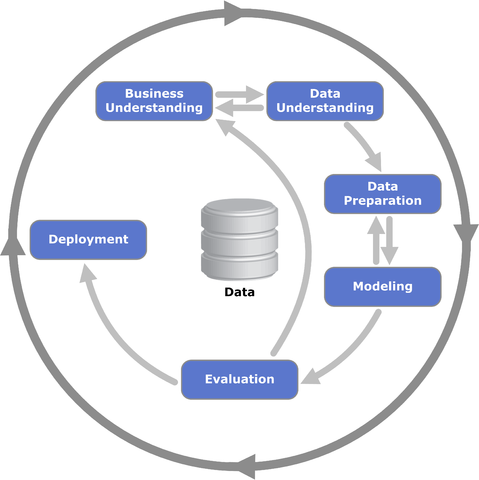
\includegraphics[width=0.5\textwidth,height=\textheight]{Data/CRISP-DM_Process_Diagram1.png}
\caption{CRISP-DM (Source:
\url{https://statistik-dresden.de/archives/1128}))}
\end{figure}

\newpage

\hypertarget{hauptteil}{%
\section{Hauptteil}\label{hauptteil}}

\hypertarget{business-understanding}{%
\subsection{Business Understanding}\label{business-understanding}}

\begin{itemize}
\tightlist
\item
  Welche Produkte werden nur in Verbindung mit anderen Produkten
  gekauft?
\item
  Welche Produkte sind zentral?
\end{itemize}

\hypertarget{laden-der-libraries}{%
\subsubsection{Laden der Libraries}\label{laden-der-libraries}}

\begin{Shaded}
\begin{Highlighting}[]
\KeywordTok{library}\NormalTok{(}\StringTok{"tidyverse"}\NormalTok{)}
\KeywordTok{library}\NormalTok{(}\StringTok{"tidygraph"}\NormalTok{)}
\KeywordTok{library}\NormalTok{(}\StringTok{"igraph"}\NormalTok{)}
\KeywordTok{library}\NormalTok{(}\StringTok{"ggraph"}\NormalTok{)}
\end{Highlighting}
\end{Shaded}

\hypertarget{importieren-der-daten}{%
\subsubsection{Importieren der Daten}\label{importieren-der-daten}}

Die Daten stammen aus der Datensatz-Bibliothek der Stanford University
und können als .txt unter folgendem Lin heruntergeladen werden. (Link:
\url{https://snap.stanford.edu/data/amazon0302.html})

Zum Einlesen der Daten kommt im Folgenden die Funktion
\textit{read.table} zum Einsatz.\\

\begin{Shaded}
\begin{Highlighting}[]
\NormalTok{amazon <-}\StringTok{ }\KeywordTok{read.table}\NormalTok{(}\StringTok{"Data/Amazon0302.txt"}\NormalTok{)}
\end{Highlighting}
\end{Shaded}

\hypertarget{data-understanding}{%
\subsection{Data Understanding}\label{data-understanding}}

Um einen ersten Einblick in die Daten zu erhalten, wird mit der Funktion
\textit{head} die ersten Zeilen des Datensatzes ausgegeben. Zusätzlich
dazu ist es von entscheidender Rolle, die Qualität der Daten zu
bewerten. Aus diesem Grund werden alle fehlenden Werte, sogenannte NAs
gezählt und ausgegeben.\\

\begin{Shaded}
\begin{Highlighting}[]
\KeywordTok{head}\NormalTok{(amazon)}
\end{Highlighting}
\end{Shaded}

\begin{verbatim}
##   V1 V2
## 1  0  1
## 2  0  2
## 3  0  3
## 4  0  4
## 5  0  5
## 6  1  0
\end{verbatim}

\begin{Shaded}
\begin{Highlighting}[]
\CommentTok{# Count NAs}
\KeywordTok{which}\NormalTok{(}\KeywordTok{is.na}\NormalTok{(amazon))}
\end{Highlighting}
\end{Shaded}

\begin{verbatim}
## integer(0)
\end{verbatim}

Der Dataframe besteht aus 3 Spalten: einer ID Spalte, und zwei
Kantenspalten. Des Weiteren weisen die Daten keine Lücken und fehlenden
Werte auf, sodass der komplette Datensatz für das weitere Vorgehen
genutzt werden kann.

\hypertarget{data-preparation}{%
\subsection{Data Preparation}\label{data-preparation}}

Auf Basis der vorangegangen Schritte müssen nun weitere Anpassungen der
Daten erfolgen, um damit arbeiten zu können. Zum Einen werden die
Kantenspalten von ihren ursprünglichen Namen in sprechendere
Bezeichnungen umbenannt. Im gleichen Schritt werden alle Werte um 1
erhöht, sodass keine Nullen mehr existieren.\\

\begin{Shaded}
\begin{Highlighting}[]
\NormalTok{dat <-}\StringTok{ }\NormalTok{amazon }\OperatorTok\StringTok{ }
\StringTok{  }\KeywordTok{rename}\NormalTok{(}
    \DataTypeTok{from =}\NormalTok{ V1,}
    \DataTypeTok{to =}\NormalTok{ V2}
\NormalTok{  ) }\OperatorTok\StringTok{ }
\StringTok{  }\KeywordTok{mutate}\NormalTok{(}
    \DataTypeTok{from =}\NormalTok{ from}\OperatorTok{+}\DecValTok{1}\NormalTok{,}
    \DataTypeTok{to =}\NormalTok{ to}\OperatorTok{+}\DecValTok{1}
\NormalTok{  )}
\end{Highlighting}
\end{Shaded}

\hypertarget{modeling}{%
\subsection{Modeling}\label{modeling}}

Nach der Datenbearbeitung kann nun das Netz gefittet werden. Hierzu wird
die Funktion \textit{as tbl graph} angewendet, um ein Netz zu
erstellen.\\

\begin{Shaded}
\begin{Highlighting}[]
\NormalTok{net <-}\StringTok{ }\KeywordTok{as_tbl_graph}\NormalTok{(dat)}
\NormalTok{net}
\end{Highlighting}
\end{Shaded}

\begin{verbatim}
## # A tbl_graph: 262111 nodes and 1234877 edges
## #
## # A directed simple graph with 1 component
## #
## # Node Data: 262,111 x 1 (active)
##   name 
##   <chr>
## 1 1    
## 2 2    
## 3 3    
## 4 4    
## 5 5    
## 6 6    
## # ... with 262,105 more rows
## #
## # Edge Data: 1,234,877 x 2
##    from    to
##   <int> <int>
## 1     1     2
## 2     1     3
## 3     1     4
## # ... with 1,234,874 more rows
\end{verbatim}

Die beiden Spalten aus dem Ursprungsdatensatz wurden in ein Netz,
bestehend aus 262111 Knoten und 1234877 Kanten, konvertiert. Es handelt
sich, wie aus der Zusammenfassung des Netzes zu entnehmen ist, um einen
gericheteten Graphen. Die Knotennamen sind in diesem Fall die Ziffern
der Kantendaten. Leider liegt dem Autor dieser Arbeit keine
Zuordnungsliste von Knotenziffern zu realen Amazonprodukten vor. Aus
diesem Grund wird im Folgenden mit den Ziffern der Knoten
weitergearbeitet.\\

\begin{Shaded}
\begin{Highlighting}[]
\CommentTok{# Calculate Degree of Vertices}
\NormalTok{degree <-}\StringTok{ }\KeywordTok{degree}\NormalTok{(net)}

\CommentTok{# Adjacency Matrix}
\NormalTok{adjacencyMatrix <-}\StringTok{ }\NormalTok{net[]}
\end{Highlighting}
\end{Shaded}

Aus dem Netz kann nun der Degree abgeleitet und abgespeichert werden.
Der Degree oder Grad eines Knoten ist die Anzahl von Kanten, die an ihn
angrenzen. Für die Analyse ist die Verteilung der Grade der Knoten
interessant. Gibt es eine überwiegende Mehrheit an Knoten, welche die
gleiche Anzahl an Kanten besitzen? Gibt es Ausreißer mit vielen Kanten?
Ähnelt die Verteilung einer Normalverteilung, ist die links oder rechts
verschoben?\\
Um diese Fragen zu beantworten, wird im nächsten Schritt ein Histogramm
erzeugt, welches die Knotengrade des Netzwerkes visualisiert.\\

\hypertarget{data-visualization}{%
\subsection{Data Visualization}\label{data-visualization}}

Um die Degrees für die Visualisierung nutzen zu können, müssen diese
zuvor in ein Dataframe umgewandelt werden. Dies geschieht mit der
Funktion \textit{as.data.frame}. Anschließend wird die Library
\textit{ggplot2} für das Histogramm angewendet.

\begin{Shaded}
\begin{Highlighting}[]
\NormalTok{degree_df <-}\StringTok{ }\KeywordTok{as.data.frame}\NormalTok{(degree)}


\NormalTok{hist_of_degrees <-}\StringTok{ }\KeywordTok{ggplot}\NormalTok{(}\DataTypeTok{data =}\NormalTok{ degree_df, }\KeywordTok{aes}\NormalTok{(}\DataTypeTok{x=}\NormalTok{degree))}\OperatorTok{+}
\StringTok{  }\KeywordTok{geom_bar}\NormalTok{(}\DataTypeTok{fill =} \StringTok{"#e2001a"}\NormalTok{, }\DataTypeTok{colour =} \StringTok{"#e2001a"}\NormalTok{, }\DataTypeTok{alpha=}\NormalTok{.}\DecValTok{5}\NormalTok{)}\OperatorTok{+}
\StringTok{  }\KeywordTok{scale_y_continuous}\NormalTok{(}\DataTypeTok{trans=}\StringTok{'log10'}\NormalTok{)}\OperatorTok{+}
\StringTok{  }\KeywordTok{xlim}\NormalTok{(}\DecValTok{0}\NormalTok{,}\DecValTok{120}\NormalTok{)}\OperatorTok{+}
\StringTok{  }\KeywordTok{labs}\NormalTok{(}\DataTypeTok{title =} \StringTok{"Histogram of Node-Degrees"}\NormalTok{, }
       \DataTypeTok{subtitle =} \StringTok{"Amazon Network Analysis"}\NormalTok{, }
       \DataTypeTok{y =} \StringTok{"Frequency (log10 scale)"}\NormalTok{, }
       \DataTypeTok{x =} \StringTok{"Degree of Vertices (xlim = 120)"}\NormalTok{)}\OperatorTok{+}
\StringTok{  }\KeywordTok{theme_classic}\NormalTok{()}

\NormalTok{hist_of_degrees}
\end{Highlighting}
\end{Shaded}

\begin{figure}
\centering
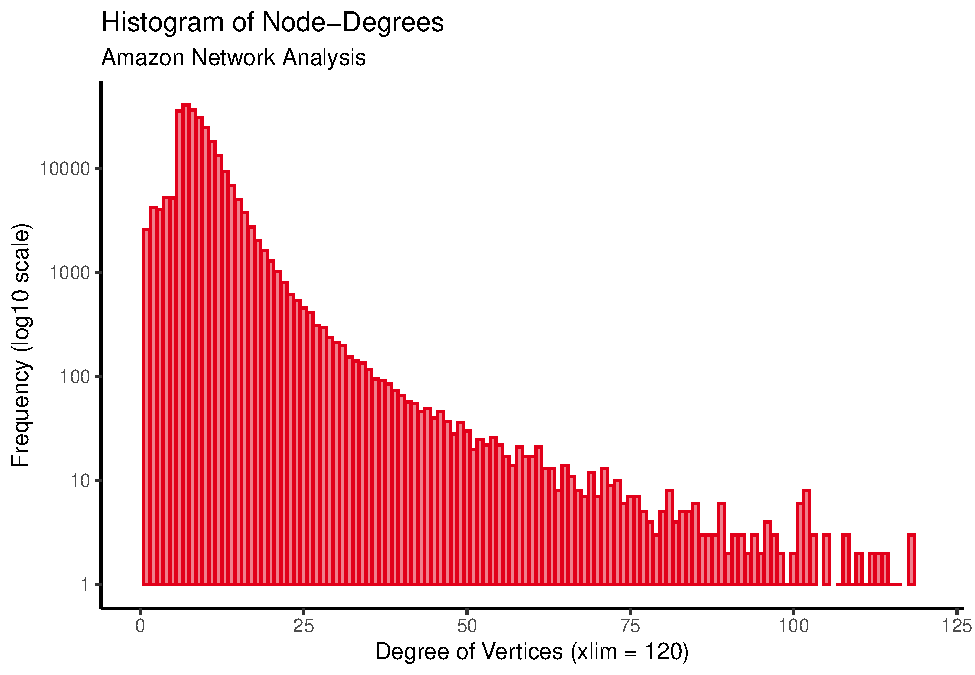
\includegraphics{Assignment_files/figure-latex/viz-1.pdf}
\caption{Knotengrad Histogramm}
\end{figure}

Das Histogramm der Knotengrade zeigt eine Mehrheit der Grade im Bereich
5-20. Dies bedeutet, dass eine Mehrheit der Knoten im Datensatz eine
durchschnittliche Anzahl an Kanten von 5-20 aufweist. Weiterhin ist zu
erkennen, dass einige Knoten 100 und mehr Kanten besitzen. Die großen
Ausreißer wurden in diesem Plot weggelassen, doch selbst in dieser
Darstellungsweise zeigt sich ein abflachender Bereich Richtung x
--\textgreater{} unendlich. Um eine übersichtlichere Darstellung der
Observationen um den Nullbereich der y-Achse zu gewährleisten, wurde die
y-Achse nach dem dekadischen Logarithmus skaliert.

\hypertarget{experimental-data}{%
\subsection{Experimental Data}\label{experimental-data}}

\begin{Shaded}
\begin{Highlighting}[]
\CommentTok{# Subsetting Data}
\NormalTok{dat_exp <-}\StringTok{ }\NormalTok{dat[}\DecValTok{1}\OperatorTok{:}\DecValTok{200}\NormalTok{,]}

\NormalTok{net_exp <-}\StringTok{ }\KeywordTok{as_tbl_graph}\NormalTok{(dat_exp)}

\NormalTok{net_exp <-}\StringTok{ }\NormalTok{net_exp }\OperatorTok\StringTok{ }
\StringTok{  }\KeywordTok{activate}\NormalTok{(nodes) }\OperatorTok\StringTok{ }
\StringTok{  }\KeywordTok{mutate}\NormalTok{(}
    \DataTypeTok{degree =} \KeywordTok{centrality_degree}\NormalTok{()}
\NormalTok{  )}
\end{Highlighting}
\end{Shaded}

\begin{Shaded}
\begin{Highlighting}[]
\CommentTok{# Data Viz for Subset}
\CommentTok{# network diagramm}
\KeywordTok{ggraph}\NormalTok{(net_exp, }\DataTypeTok{layout =} \StringTok{'fr'}\NormalTok{, }\DataTypeTok{maxiter =} \DecValTok{100}\NormalTok{) }\OperatorTok{+}\StringTok{ }
\StringTok{  }\KeywordTok{geom_node_point}\NormalTok{(}\DataTypeTok{colour=}\StringTok{"#e2001a"}\NormalTok{) }\OperatorTok{+}\StringTok{ }
\StringTok{  }\KeywordTok{geom_edge_link}\NormalTok{(}\DataTypeTok{alpha =} \FloatTok{.4}\NormalTok{) }\OperatorTok{+}
\StringTok{  }\KeywordTok{theme_graph}\NormalTok{()}
\end{Highlighting}
\end{Shaded}

\begin{figure}
\centering
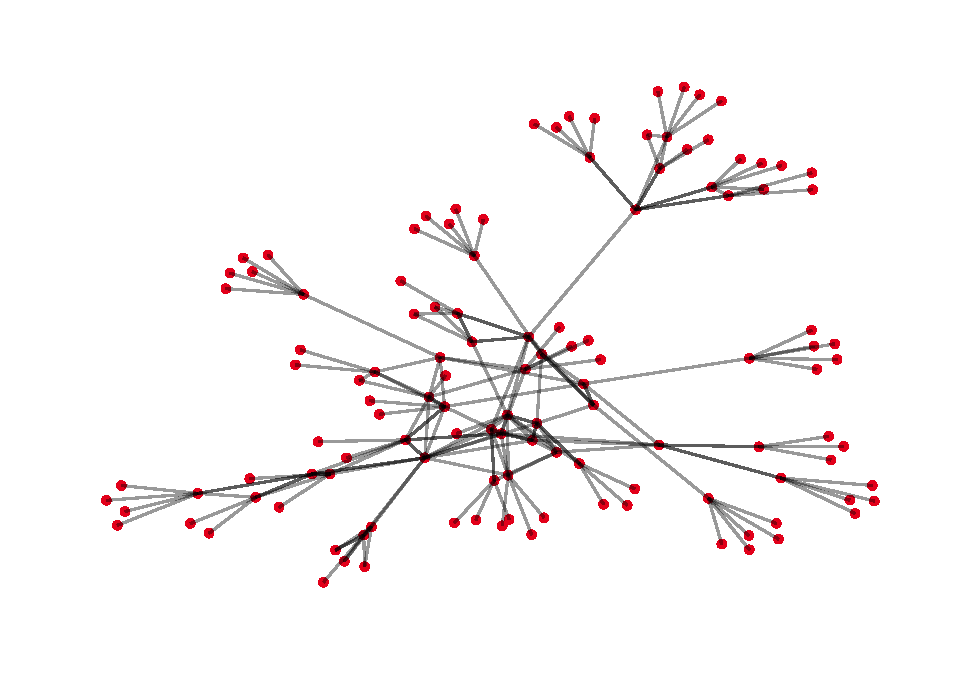
\includegraphics{Assignment_files/figure-latex/unnamed-chunk-2-1.pdf}
\caption{Netzwerk Visualisierung 1}
\end{figure}

\begin{Shaded}
\begin{Highlighting}[]
\KeywordTok{ggraph}\NormalTok{(net_exp, }\DataTypeTok{layout =} \StringTok{'kk'}\NormalTok{, }\DataTypeTok{maxiter =} \DecValTok{100}\NormalTok{) }\OperatorTok{+}\StringTok{ }
\StringTok{  }\KeywordTok{geom_node_point}\NormalTok{(}\DataTypeTok{colour=}\StringTok{"#e2001a"}\NormalTok{) }\OperatorTok{+}\StringTok{ }
\StringTok{  }\KeywordTok{geom_edge_link}\NormalTok{(}\DataTypeTok{alpha =} \FloatTok{.4}\NormalTok{) }\OperatorTok{+}
\StringTok{  }\KeywordTok{theme_graph}\NormalTok{()}
\end{Highlighting}
\end{Shaded}

\begin{figure}
\centering
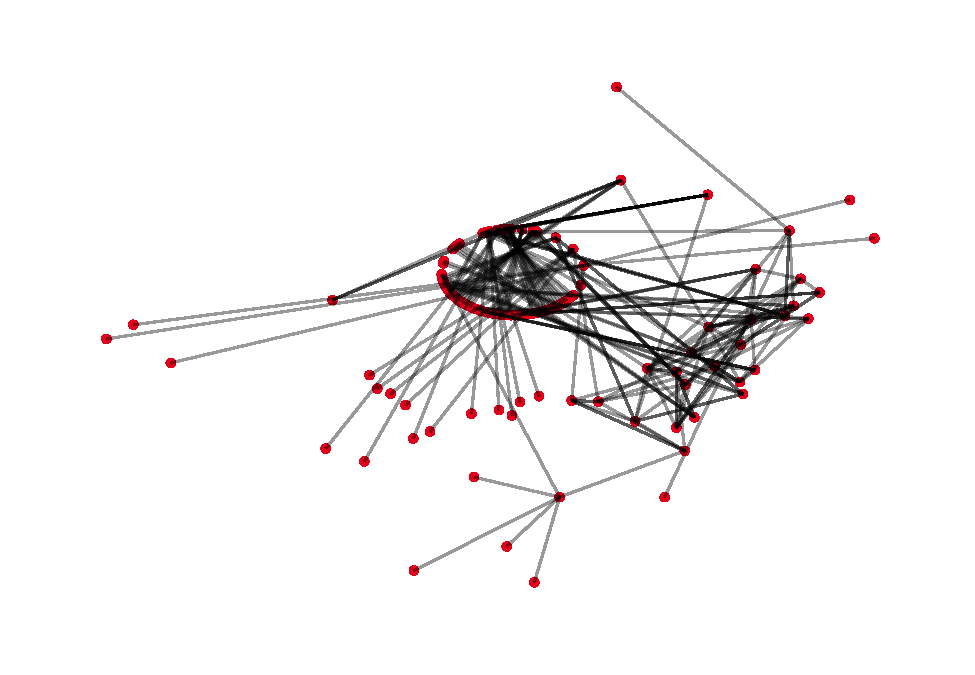
\includegraphics{Assignment_files/figure-latex/unnamed-chunk-3-1.pdf}
\caption{Netzwerk Visualisierung 2}
\end{figure}

\begin{Shaded}
\begin{Highlighting}[]
\CommentTok{# coord diagramm}
\KeywordTok{ggraph}\NormalTok{(net_exp, }\DataTypeTok{layout =} \StringTok{'linear'}\NormalTok{, }\DataTypeTok{circular =} \OtherTok{TRUE}\NormalTok{) }\OperatorTok{+}\StringTok{ }
\StringTok{  }\KeywordTok{geom_node_point}\NormalTok{(}\DataTypeTok{colour=}\StringTok{"#e2001a"}\NormalTok{) }\OperatorTok{+}
\StringTok{  }\KeywordTok{geom_edge_arc}\NormalTok{(}\DataTypeTok{alpha =} \FloatTok{.4}\NormalTok{) }\OperatorTok{+}
\StringTok{  }\KeywordTok{theme_graph}\NormalTok{()}
\end{Highlighting}
\end{Shaded}

\begin{figure}
\centering
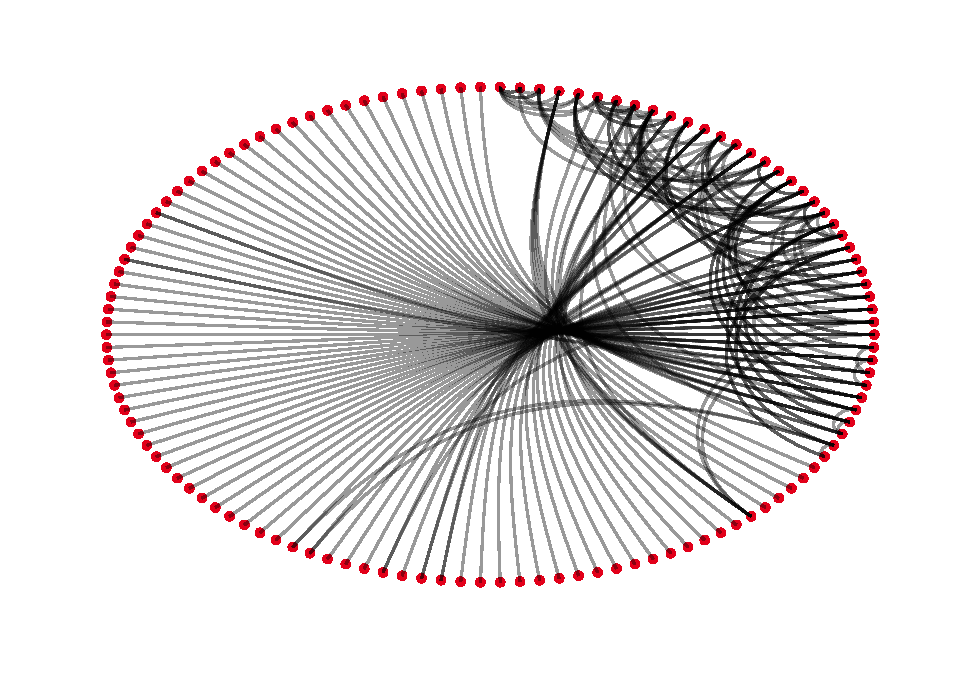
\includegraphics{Assignment_files/figure-latex/unnamed-chunk-4-1.pdf}
\caption{Netzwerk Visualisierung 3}
\end{figure}

\newpage

\hypertarget{fazit}{%
\section{Fazit}\label{fazit}}

\hypertarget{evaluation-der-ergebnisse}{%
\subsection{Evaluation der Ergebnisse}\label{evaluation-der-ergebnisse}}

tbd

\hypertarget{kritische-reflexion}{%
\subsection{kritische Reflexion}\label{kritische-reflexion}}

tbd

\end{document}
